\documentclass{patmorin}
\usepackage{amsthm,amsmath,graphicx,stmaryrd}
\usepackage{pat}

\DeclareMathOperator{\erf}{erf}
\newcommand{\eps}{\varepsilon}

\title{\MakeUppercase{On the Average Number of Edges in a Theta Graph}}
\author{Pat Morin,\thanks{School of Computer Science, Carleton University}\,\,
         and Sander Verdonschot\footnotemark[1]}



\begin{document}
\maketitle

\begin{abstract}
  The abstract goes here.
\end{abstract}

\section{Introduction}

In this paper, we study the average number of edges in a $\theta$-graph
of a random point set.  A typical model for random point sets is a set
of $n$ points independently and uniformly distributed in $[0,1]^2$.
In this paper, however, we will consider points generated by a
homogeneous Poisson process with unit intensity over the entire
plane, $\R^2$.  In this model, the number of points in any region
whose area is $A$ follows a Poisson distribution with parameter $A$.
For definitions of Poisson processes and distributions see, for example,
Ross \cite[Chapter~2]{ross:introduction}.  For our purposes, the most
important properties of the Poisson process are the following
\begin{enumerate}
\item The probability  that a particular region $X$ whose area is $A$
   is empty of points is exactly $e^{-A}$.
\item For two disjoint regions $X$ and $Y$, the events ``$X$ is empty
   of points'' and ``$Y$ is empty of points'' are independent.
\end{enumerate}
Note that, in this model, any $\theta$-graph will have an infinite number
of edges since there are an infinite number of points.  Therefore,
we study the average degree of a vertex in the $\theta$-graph.  For the
$\theta_k$-graph, this quantity is at most $2k$ since each vertex defines
$k$ edges of the graph and each edge has 2 endpoints.  However, in some
cases an edge $uw$ is \emph{mutual} in the sense that the edge is created
both by $u$ and by $w$.  If we let $p_k$ denote the probability that an
edge of the $\theta_k$ graph is is mutual, then the average degree of
the $\theta_k$ graph is
\[
    d_k = (2-p_k)k \enspace .
\]
Thus, understanding the average degree of a $\theta_k$ graph boils down
to computing $p_k$.

\section{An Analysis of $\theta_k$ for even $k$}

In this section we determine the value of $p_k$ for even values of $k$.
Surprisigly, the value of $p_k$ in this does not depend on $k$.

\begin{lem}
 For even integers $k\ge 4$, $p_k=\frac{\pi\sqrt{3}}{9}\approx 0.6045997883$.
\end{lem}

\begin{proof}
  Let $u$ be an arbitrary vertex in a $\theta_k$ graph and let $w$
  be a vertex that $u$ has chosen as a neighbour in one of its cones,
  $C$ ($w$ is the ``closest'' vertex to $u$ in $C$).  Let $T$ be the
  open isosceles triangle defined by $C$ and a line
  through $w$ that is orthogonal to the axis of $C$. See \figref{mutual}.
  Observe that the location of $w$ is uniformly distributed on the
  edge of $T$ opposite $u$;  if this edge has length $\ell$, then $w$
  partitions it into two pieces of length $r$ and $\ell-r$, where $r$
  is uniformly distributed in $[0,\ell]$.

  \begin{figure}
    \centering{\includegraphics{cone}}
    \caption{The edge $uw$ is mutual if and only if $T'\setminus T$ 
       is empty of points.}
    \figlabel{mutual}
  \end{figure}
 
  Let $T'$ be the triangle obtained by reflecting $T$ through the midpoint
  of the edge $uw$ (so that $w$ is a vertex of $T'$). By Property~2 of the
  Poisson process, the edge $uw$ is mutual if and only if $T'\setminus T$
  contains no points.  The area of $T'\setminus T$ is
  \[
     A(T'\setminus T) = c(r^2+(\ell-r)^2)  \enspace ,
  \]
  where $c=c(k)$ depends only on $k$.  We now have enough information
  to compute the probability that the edge $uw$ is mutual conditional
  on $\ell$ and $r$:
  \[
    \Pr\{\mbox{$uw$ is mutual} \mid l,r\} = \exp(-c(r^2+(\ell-r)^2))
      \enspace .
  \]
  Since $r$ (conditioned on $\ell$) is uniform over $[0,\ell]$, unconditioning
  $r$ gives
  \begin{align*}
    f(\ell) & \equiv \Pr\{\mbox{$uw$ is mutual} \mid l\} \\
     & = \int_0^\ell (1/\ell)\exp(-c(r^2+(\ell-r)^2))\,\mathrm{d}r \\
     & = \frac{\sqrt{\pi}}{\ell\sqrt{2c}}
            \cdot\exp(-c\ell^2/2)
            \cdot\erf(\ell\sqrt{c/2})  \enspace ,
%     & = \sqrt{\frac{2\pi}{\sqrt{3}}}\exp(-\sqrt{3}\ell^2/8)
%         \cdot\erf(\sqrt[4]{3}\sqrt{2}\ell/4) \enspace ,
  \end{align*}
  where 
  \[ \erf(x)=\frac{2}{\sqrt{\pi}}\int_0^x e^{-t^2}\,\mathrm{d}t \]
  is the \emph{Gauss error function} \cite{gauss-error}.  (The derivation
  of the integrals and derivatives in this proof using Maple are given
  in \appref{derivations}.)

  Next, we remove the conditioning on $\ell$.  The triangle $T$ defines a
  region of area $c\ell^2$ that is empty of points.  Therefore,
  by Property~1 of the Poisson process, the cumulative distribution
  function of $\ell$ is given by
  \[
    P(x) \equiv \Pr\{\ell \le x\} = 1-\exp(-cx^2) \enspace .
  \]
  The probability density function of $\ell$ is therefore given by 
  \[
     p(x) \equiv \frac{d}{dx}P(x) =
     2cx\cdot\exp(-cx^2) \enspace .
  \]
  Finally, we obtain $p_k$ as 
  \begin{align*}
     p_k = \int_0^\infty p(\ell)\cdot f(\ell)\,\mathrm{d}\ell 
     = \frac{\pi\sqrt{3}}{9}
      \approx 0.6045997883  \enspace . & \qedhere
  \end{align*}
\end{proof}

Thus, for even $k$, the average degree of the $\theta_k$-graph is 
\[ d_k = \left(2-\frac{\pi\sqrt{3}}{9}\right)k \approx 1.395400212k \enspace . \]

\section{The Second Section}

\section{Summary}
\seclabel{summary}

\section*{Acknowledgement}

The authors of this paper are partly funded by NSERC and CFI.

\bibliographystyle{plain}
\bibliography{template}

\appendix

\section{Derivations in Maple}
\applabel{derivations}

\noindent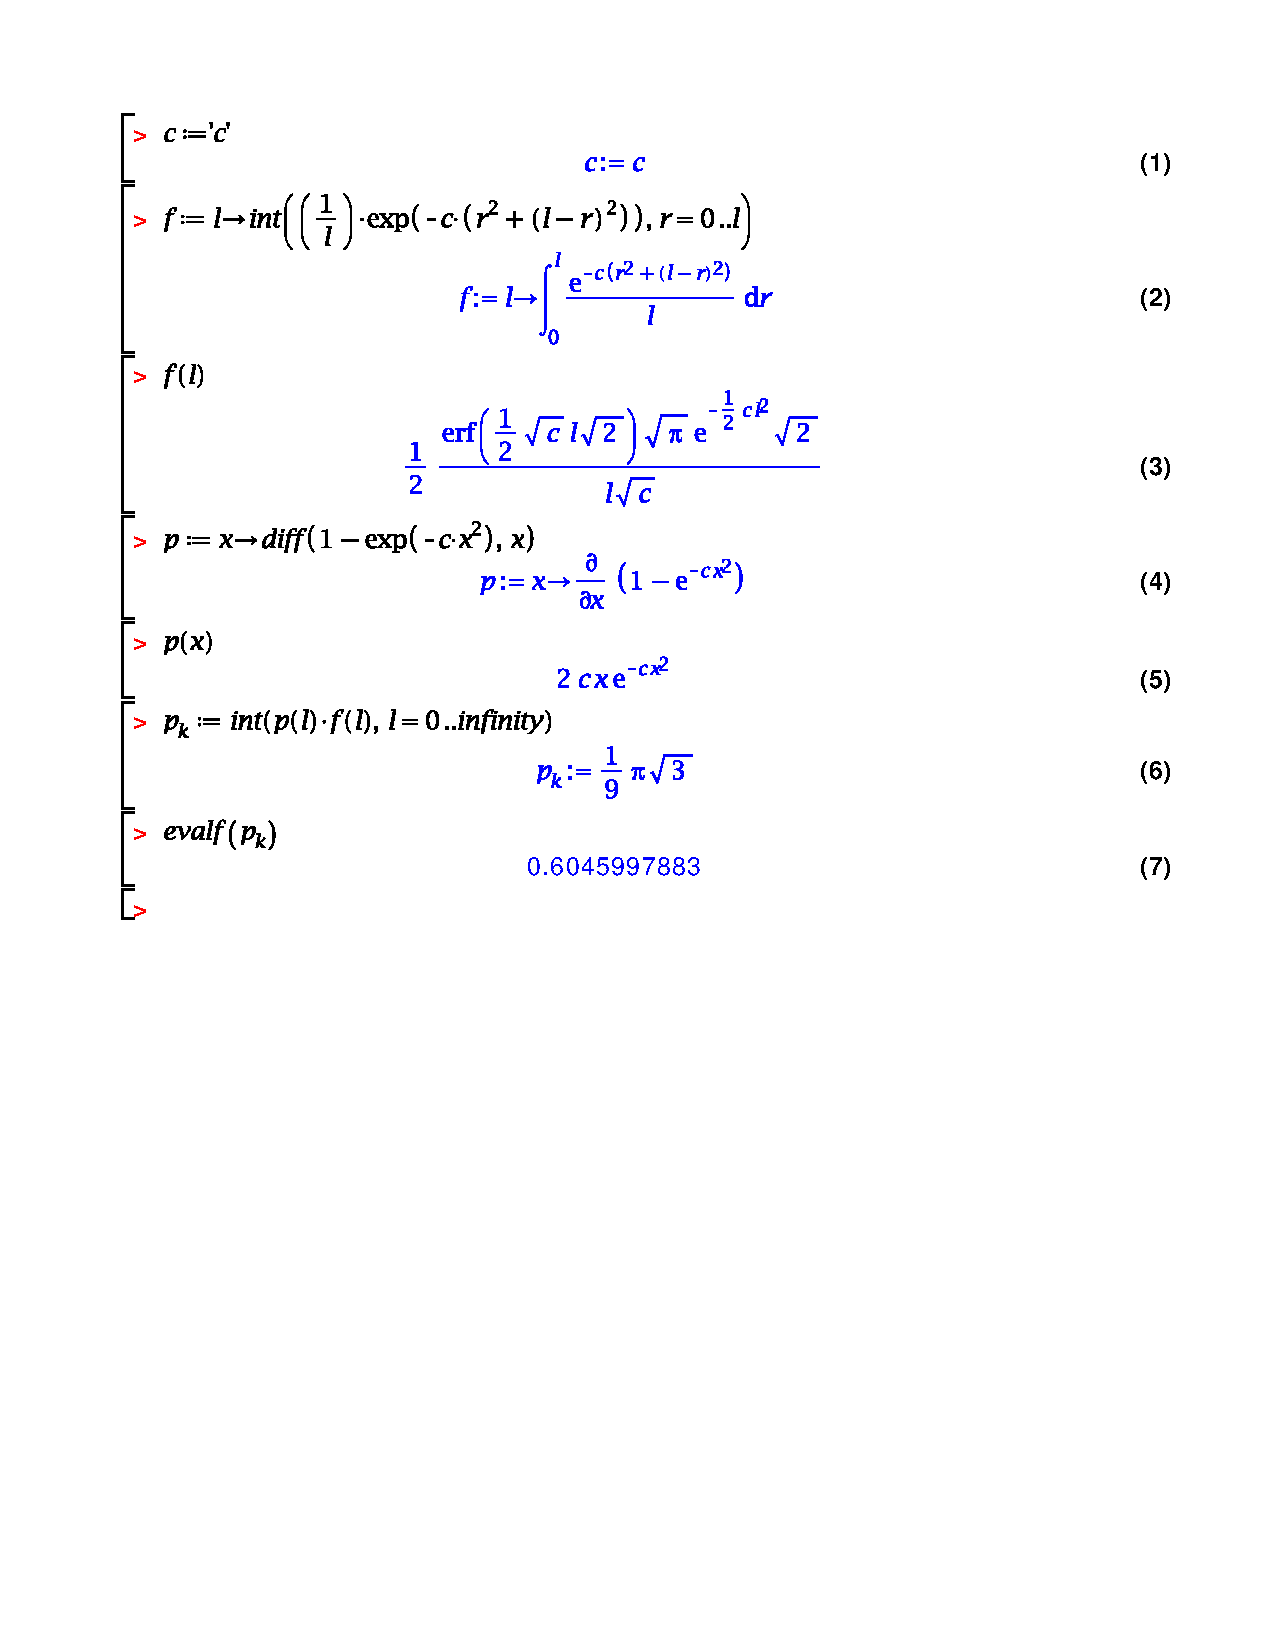
\includegraphics{even}



\end{document}


